\documentclass{beamer}
\usepackage[spanish]{babel}
\usepackage[dvipsnames]{xcolor}
\usepackage{tikz}
\usepackage{hyperref}
%Declaracion del tema modificado
\usetheme[logo=rpi]{arturo}
%Declaracion de contenedor de imagenes
\graphicspath{{images/}}
%--------------------------------------
\title{Curso básico-intermedio de programación en Raspberry Pi}
\subtitle{Curso intersemestral}
\date{\today}
\author[OACM]{M.I Omar Arturo Castillo Méndez} 

\begin{document}
	
	\begin{frame}[plain]
		\titlepage
	\end{frame}
	
	\begin{frame}{Contenido}
		\tableofcontents
	\end{frame}
	
	\section{Introducción}
	
	\begin{frame}{Introducción}
		\framesubtitle{Examen de diagnostico}
		\begin{itemize}
			\item ¿Qué es una tarjeta Raspberry Pi?
			\item Si conoces algún lenguaje de programación, ¿Cuál o cuáles?
			\item ¿Qué es el lenguaje de programación Python?
			\item ¿Qué bibliotecas de Python conoces?
			\item En la configuración de puertos de una RPi, ¿Qué diferencia hay entre el BCM y BOARD?
			\item Escriba un código para encender un LED en una tarjeta Raspberry Pi usando la configuración de puertos BOARD.
			\item ¿Cuáles son tus expectativas del curso?
		\end{itemize}
	\end{frame}
	
	\begin{frame}
		\frametitle{Introducción}
		\framesubtitle{¿Qué es una Raspberry Pi?}
		Es una tarjeta de desarrollo, diseñada como una computadora modular, con una arquitectura ARM y usando un sistema operativo basado en Linux (Raspbian OS).
		\begin{figure}
			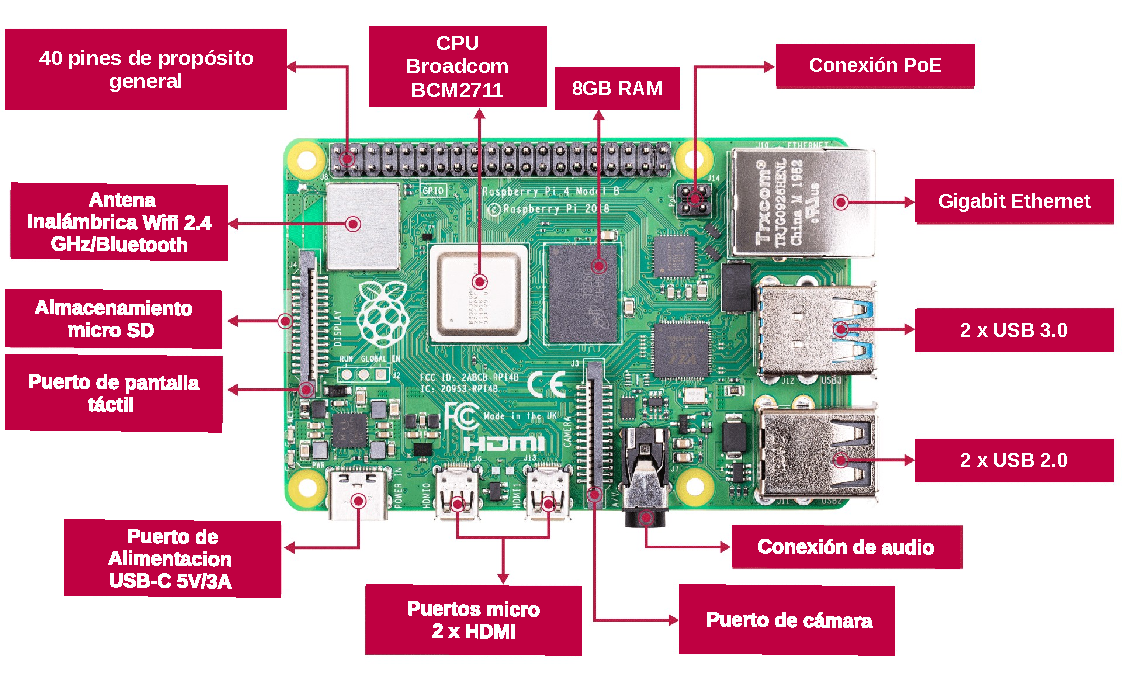
\includegraphics[scale=0.4]{rpiboard}
			\caption{Tarjeta Raspberry Pi 4}
		\end{figure}
		
	\end{frame}	

	\section{Configuración}
	\begin{frame}
		\frametitle{Configuración inicial}
		\framesubtitle{Requisitos}
		
		\begin{tcolorbox}[enhanced, title= Material necesario:]
			\begin{itemize}
				\item Tarjeta Raspberry Pi(Cualquier versión)
				\item Fuente de alimentación de 5V a 3A
				\item Tarjeta de almacenamiento micro SD de 64 Gb o superior clase 10 o superior
			\end{itemize}
		\end{tcolorbox}
		
			
	\end{frame}

	\begin{frame}
		\frametitle{Configuración inicial}
		\framesubtitle{Instalación de Raspbian}
		
		\begin{tcolorbox}[enhanced, title= Instrucciones:]
				\begin{itemize}
					\item Visitar la siguiente liga: \url{https://www.raspberrypi.com/software/}
					\item Descargar la version correspondiente con su respectivo sistema operativo, y dar click en \textbf{descargar}
					\item Una vez instalado se mostrará la siguiente interfaz de Raspberry Pi Imager.
				\end{itemize}
		\end{tcolorbox}
		
		
	\end{frame}
	
	\begin{frame}
		\frametitle{Configuración inicial}
		\framesubtitle{Instalación de Raspbian}	
		
		\begin{figure}
			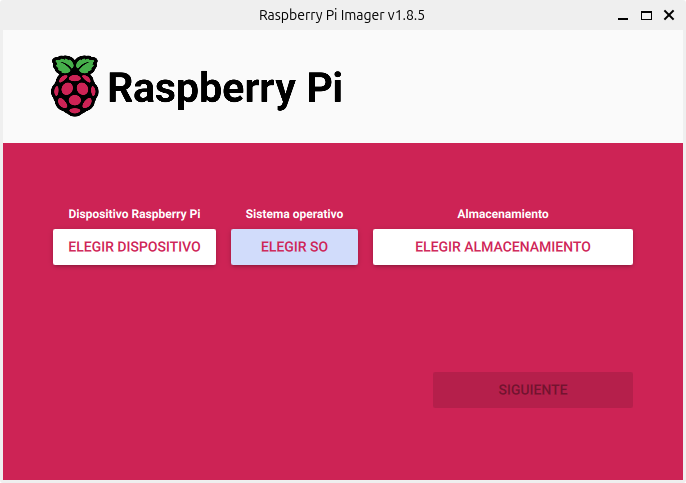
\includegraphics[scale=0.35]{imager.png}
			\caption{Interfaz: Raspberry Pi Imager}
		\end{figure}
		
	\end{frame}
	
	\begin{frame}
		\frametitle{Configuración inicial}
		\framesubtitle{Selección de Tarjeta}
		
		\begin{figure}
			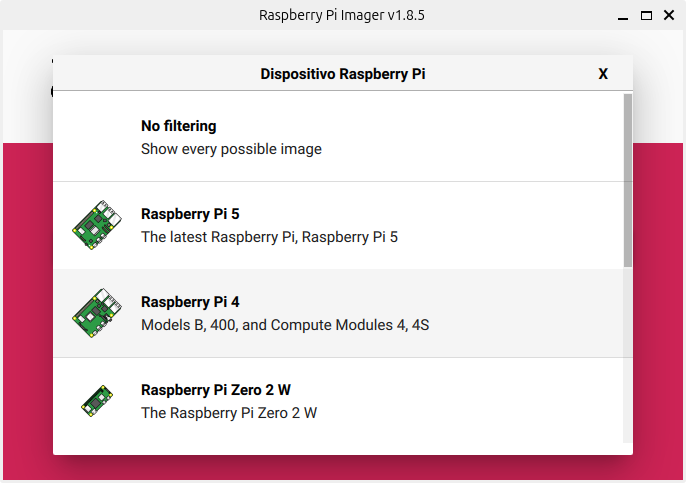
\includegraphics[scale=0.35]{imager2.png}
			\caption{Selección de tarjeta Raspberry Pi}
		\end{figure}
		
	\end{frame}
	
	\begin{frame}
		\frametitle{Configuración inicial}
		\framesubtitle{Selección de sistema operativo}
		
		\begin{figure}
			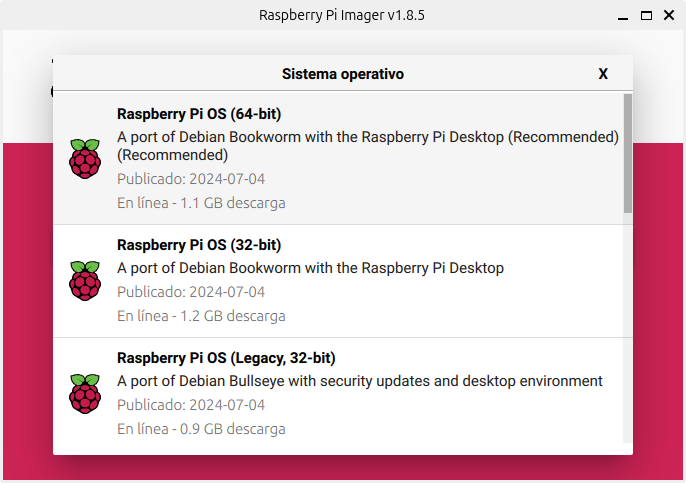
\includegraphics[scale=0.35]{imager3.png}
			\caption{Selección de sistema operativo}
		\end{figure}
		
	\end{frame}
	
	\begin{frame}
		\frametitle{Configuración inicial}
		\framesubtitle{Selección de unidad de almacenamiento}
		
		\begin{figure}
			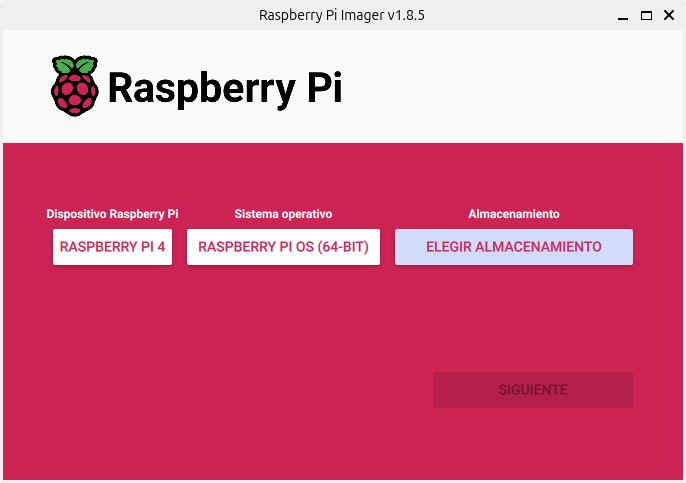
\includegraphics[scale=0.35]{imager4.png}
			\caption{Selección de unidad de almacenamiento}
		\end{figure}
		
	\end{frame}
	
	\section{Comandos básicos}
	\begin{frame}
		\frametitle{Comandos básicos de la terminal}
		
		\begin{tcolorbox}[enhanced, title= Instrucciones:]
			\begin{itemize}
				\item cd  : Cambiar de directorio a una ruta especificada.
				\item cd .. : Subir un nivel en la ruta.
				\item ls  : Listar archivos de un fichero/carpeta.
				\item pwd : Mostrar la ruta del carpeta.
				\item mkdir : Crear una carpeta.
				\item nano : Gestor de texto desde la terminal.
				\item cp   : Copiar fichero o archivo hacia una ruta especificada. 
			\end{itemize}
		\end{tcolorbox}
		
	\end{frame}
	
%----------------------------------------------------
\end{document}